
\documentclass[12pt]{article}
\usepackage{lmodern}
\usepackage{graphicx}
\usepackage{caption}
\usepackage{amssymb}
\usepackage{amsmath}
\DeclareMathOperator\cis{cis} % Added 'cis' as a function to amsmath
\DeclareMathOperator\Arg{Arg} % Added 'Arg' as a function to amsmath
\usepackage{bm}
\usepackage{wasysym}
\usepackage{latexsym}

\usepackage{tikz}
\usepackage{pgfplots}

\pgfplotsset{width=6.5cm,compat=1.13}

\usepgfplotslibrary{polar}%adds polar axes library and environment to TeX for easier polar representations of Data

\usepackage[multiple]{footmisc}

\usepackage{enumitem}

\usepackage[colorlinks=true,linkcolor=blue,citecolor=blue]{hyperref}
% FIXED FOOTNOTES [multiple] option conflict with Hyperref!!!!!!
\let\oldFootnote\footnote
\newcommand\nextToken\relax

\renewcommand\footnote[1]{%
    \oldFootnote{#1}\futurelet\nextToken\isFootnote}

\newcommand\isFootnote{%
    \ifx\footnote\nextToken\textsuperscript{,}\fi}

\usepackage[margin=1in,includefoot]{geometry}
\usepackage{fancyhdr}
\pagestyle{fancy}
\fancyhead{}
\fancyhead[R]{\thepage\ }
\fancyfoot{}
\renewcommand{\headrulewidth}{0pt}
\renewcommand{\footrulewidth}{0pt}
\usepackage[nottoc,notlot,notlof]{tocbibind}

\usepackage{subcaption}

\setlist[enumerate,1]{start=0}

\begin{document}
\sffamily
\begin{titlepage}
\begin{center}

\Huge{W.H.S Mathematics Presentation}\\
\LARGE{Think about Mathematics and Physics naturally}\\
[45mm]

\LARGE{By: Michael Gonzalez\\
[5mm]
Prof. Ramirez's SP 2018 3rd pd. Physics}\\
[5mm]

April $\text{4}^{\text{th}}$, 2018 \\
\end{center}
\end{titlepage}

\pagenumbering{roman}

\cleardoublepage

\section*{Notation, Formulas, and Equations}\label{sec:Formulas}
\addcontentsline{toc}{section}{\numberline{}Notation, Formulas and Equations}

Notation should be pretty standard complex analysis notation\footnote{Actual notation used comes from this book: Joseph Bak, Donald J.
Newman, 'Complex Analysis', 3rd ed.}. The space of complex numbers is denoted $\mathbb{C}$, by convention, the variable used to denote a 
function of a complex variable the letter $z$ is used.

\[ z := x + iy, \; \forall z\in \mathbb{C}; \quad \Re{z} = x; \quad \Im{z} = y; \quad \lVert z\rVert = \sqrt{x^2 + y^2};\]

Polar representation of complex numbers requires information about the angle a complex number $z$ makes with the positive $\mathbb{R}$
-axis, for this discussion. The angle $\theta$ a complex number $z$ makes is called the argument of the number $z$:

\[ \Arg{z} = \theta = \arccos{\frac{\Re{z}}{\lVert z \rVert}} = \arcsin{\frac{\Im{z}}{\lVert z \rVert}} = \arctan{\frac{\Im{z}}{\Re{z}}} + \gamma; \]

where $\gamma$:

\[ \gamma \iff \pi,\;\{x<0,\;y>0\}, \quad \text{or} \quad \{x<0, \; y<0\};\]
\[ \gamma \iff 2\pi,\;\{x>0,\;y<0\};\] 

The complete polar representation of a complex number $z$ below:

\[ r = \lVert z \rVert; \quad \cis{\theta} = \cos{\theta} + i\sin{\theta}; \quad z = r\cis{\theta};\]

These tools are used in the presentation for the proof outlined.

\cleardoublepage

\tableofcontents
\thispagestyle{empty}
\cleardoublepage

\pagenumbering{arabic}
\setcounter{page}{1}
\section{Introduction}\label{sec:Intro}

Physics uses mathematical descriptions to model events in the physical world. Consequentially, a firm foundation in mathematics is useful to the modern physicist. Today I am here to explain another way to think about mathematics to facilitate learning more difficult problems.

\section{Roots of Complex Numbers}

The complex plane imposes interesting results due to the structure of the numbers in the space. Notably, the entire complex plane is
isomorphic\footnote{Not sure if correct term to use here.} to the space $\mathbb{R}^2$, the cartesian plane, the complex numbers cannot 
have an 'traditional' binary order operation, and complex numbers lend themselves to vector equations/operations. All the implications of 
the structure of the complex numbers are out of scope for now, I want to introduce an interesting problem to solve from the complex plane.

There are two conventional ways of representing the complex numbers in mathematics: cartesian, and polar representation. The cartesian representation is straightforward:

\begin{tikzpicture}

	\begin{axis}[axis lines = left,
	 xlabel = {$x(\Re{z})$},
	 ylabel = {$iy(\Im{z})$},
	 xmin=0, xmax=5,
	 ymin=0, ymax=5,
	 xtick={0,...,4},
	 ytick={0,...,4}]
		\addplot[color=black] coordinates{(0,0)(1.5,1)}; % adds black line, no markers
		\addplot[color=black, mark=*] coordinates{(1.5,1)}; % adds black marker to specified point for emphasis, this is a Complex number
		\addplot[color=black] coordinates{(0,0)(2,3)};
		\addplot[color=black, mark=*] coordinates{(2,3)};
	\end{axis}

\end{tikzpicture}% Removes whitespace between axes!!!
\hskip 10pt
\begin{tikzpicture}
	\begin{axis}[axis lines = left,
	 xlabel = {$x(\Re{z})$},
	 ylabel = {$iy(\Im{z})$},
	 xmin=0, xmax=5,
	 ymin=0, ymax=5,
	 xtick={0,...,4},
	 ytick={0,...,4}]
	 	\addplot[color=black,quiver={u=\thisrow{u},v=\thisrow{v}}, -stealth,] table{
	 		x y u v
	 		0 0 0 0
	 		0 0 1.5 1
	 		0 0 0 0
	 		0 0 2 3
	 	};
	\end{axis}
\end{tikzpicture}

The polar representation uses angles and lengths to represent the same complex numbers.

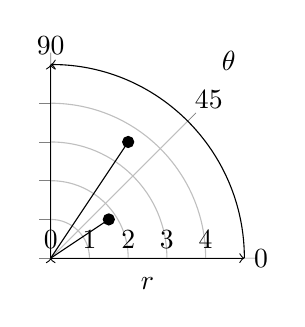
\begin{tikzpicture}

	\begin{polaraxis}[xmin=0, xmax=90,
	ymin=0, ymax=5,
	axis line style = {->},
	y label style={at={(axis description cs:0.5,-0.05)},anchor=north},
	x label style={at={(axis description cs:0.9192388153,0.9192388153)},rotate=45,anchor=south},
	ylabel={$r$},
	xlabel={$\theta$},
	ytick={0,...,4}]
		\addplot[data cs=cart, color=black] coordinates{(0,0)(1.5,1)};
		\addplot[data cs=cart, color=black, mark=*] coordinates{(1.5,1)};
		\addplot[data cs=cart, color=black] coordinates{(0,0)(2,3)};
		\addplot[data cs=cart, color=black, mark=*] coordinates{(2,3)};
	\end{polaraxis}

\end{tikzpicture}

The type of problem I want to solve is best solved via the polar representation of complex numbers.

\cleardoublepage

\end{document}
